\documentclass{article}

\usepackage[spanish]{babel}

% Set page size and margins
% Replace `letterpaper' with `a4paper' for UK/EU standard size
\usepackage[letterpaper,top=2cm,bottom=2cm,left=3cm,right=3cm,marginparwidth=1.75cm]{geometry}

% Useful packages
\usepackage{amsmath}
\usepackage{graphicx}
\usepackage[colorlinks=true, allcolors=blue]{hyperref}

\title{Practica 4 TALF}
\author{José Ruiz Pareja}

\begin{document}
\maketitle


\section{Implementa un programa WHILE que calcule la suma de tres valores}

He definido el siguiente programa WHILE:

\begin{verbatim}
Q: (3, 4, s)
s:
X4 := 0;

while X1 != 0 do
    X4 := X4 + 1;
    X1 := X1 - 1
od;

while X2 != 0 do
    X4 := X4 + 1;
    X2 := X2 - 1
od;

while X3 != 0 do
    X4 := X4 + 1;
    X3 := X3 - 1
od;

X1 := X4

\end{verbatim}

\newpage

\subsection{Ejecútala con el compilador de WHILE y halla $T_Q$(3, 5, 2)}


Donde usamos X4 como variable auxiliar para acumular el resultado de la suma. 
Si cargamos el programa e introducimos las variables (3,5,2) podemos ver el resultado de la suma y $T_Q$(3,5,2).


\begin{center}
    \centering
    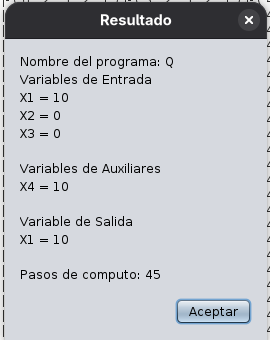
\includegraphics[width=0.5\linewidth]{imagen1.png}
\end{center}

Como podemos ver el resultado de la suma es el valor asignado a la variable X1 (10), y

\begin{center}
$T_Q(3,5,2) = 45$
\end{center}


\subsection{Ejecútala en Python y comprueba que coincide.}

Primero definimos el programa de la siguiente forma:

\begin{verbatim}
    Q="(3,X4:=0; while X1!=0 do X4:=X4+1; X1:=X1-1 od; while X2!=0 do X4:=X4+1; 
    X2:=X2-1 od; while X3!=0 do X4:=X4+1; X3:=X3-1 od; X1:=X4)"
\end{verbatim}

Y ejecutamos las funciones $f\_function(Q,[3,5,2])$ y $t\_steps(Q,[3,5,2])$ para averiguar el valor resultante y la complejidad temporal del programa con la entrada (3,5,2)

\begin{center}
    \centering
    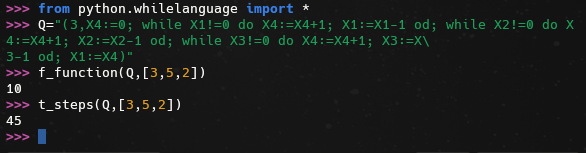
\includegraphics[width=0.5\linewidth]{imagen2.png}
\end{center}

\newpage

\section{Crea el programa WHILE más sencillo que calcule la función diverge (con cero argumentos) y calcula la codificación de su código.}

Primero definimos el siguiente programa WHILE:

\begin{verbatim}
    P=(0, 1, s)
    s:
    X1:=X1 + 1
    while X1!=0 do 
        X1:=X1 
    od
\end{verbatim}


Que sería un bucle infinito, por lo que divergería siempre ya que no tiene variables de entrada.

Usamos la funcion $while2n$ en python para averiguar la codificacion del programa WHILE

\begin{center}
    \centering
    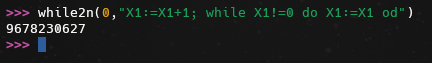
\includegraphics[width=0.5\linewidth]{imagen3.png}
\end{center}

Como podemos ver la codificacion del codigo es $9678230627$

\section{Crea una función de Python que enumere los k primeros vectores de N\text{*}}

La funcion definida es:

\begin{verbatim}
    
from .godeldecoding import godeldecoding

def enumN(n: int) -> int:
    res=[]
    for i in range(n):
        res.append(godeldecoding(i))
    return res
\end{verbatim}

Que si la probamos en terminal vemos que funciona:

\begin{center}
    \centering
    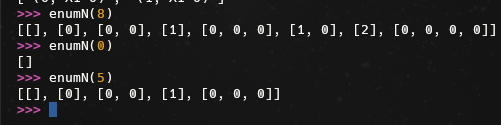
\includegraphics[width=0.5\linewidth]{imagen4.png}
\end{center}

\newpage

\section{Crea una función de Python que enumere los k primeros programas WHILE.}

La funcion definida es:

\begin{verbatim}
from .n2while import n2while


def enumWhile(n: int) -> str:
    res=[]
    for i in range(n):
        res.append(n2while(i))
    return res


\end{verbatim}

Que si la probamos en terminal vemos que funciona:

\begin{center}
    \centering
    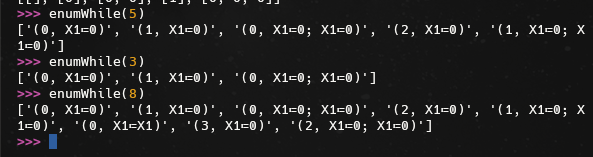
\includegraphics[width=0.5\linewidth]{imagen5.png}
\end{center}


\end{document}
